%%%%%%%%%%%%%%%%%%%% book.tex %%%%%%%%%%%%%%%%%%%%%%%%%%%%%
%
% sample root file for the chapters of your "monograph"
%
% Use this file as a template for your own input.
%
%%%%%%%%%%%%%%%% Springer-Verlag %%%%%%%%%%%%%%%%%%%%%%%%%%


% RECOMMENDED %%%%%%%%%%%%%%%%%%%%%%%%%%%%%%%%%%%%%%%%%%%%%%%%%%%
\documentclass[pdftex,12pt, oneside]{book}
 
% choose options for [] as required from the list
% in the Reference Guide, Sect. 2.2
%\usepackage[paperwidth=8.5in, paperheight=13in]{geometry} %Folio
\usepackage[paperwidth=8.27in, paperheight=11.69in]{geometry} %A4

\usepackage{makeidx}         % allows index generation
\usepackage{graphicx}        % standard LaTeX graphics tool
                             % when including figure files
\usepackage[bottom]{footmisc}% places footnotes at page bottom
\usepackage[bahasa]{babel}
\usepackage{enumerate}
\usepackage{paralist}
\usepackage{float}
\usepackage{gensymb}  
\usepackage{listings}
\usepackage{color}
\renewcommand{\baselinestretch}{1.5}

\newcommand{\HRule}{\rule{\linewidth}{0.5mm}}

\makeindex             % used for the subject index
                       % please use the style svind.ist with
                       % your makeindex 
                     
\definecolor{codegreen}{rgb}{0,0.6,0}
\definecolor{codegray}{rgb}{0.5,0.5,0.5}
\definecolor{codepurple}{rgb}{0.58,0,0.82}
\definecolor{backcolor}{rgb}{0.95,0.95,0.92}

\lstdefinestyle{mystyle}{
  backgroundcolor=\color{backcolor},
  commentstyle=\color{codegreen},
  keywordstyle=\color{magenta},
  stringstyle=\color{codepurple},
  basicstyle=\footnotesize,
  breakatwhitespace=false,
  breaklines=true,
  captionpos=b,
  keepspaces=true,
  numbers=left,
  numbersep=5pt,
  showspaces=false,
  showstringspaces=false,
  showtabs=false,
  tabsize=2
}

\lstset{style=mystyle}


%%%%%%%%%%%%%%%%%%%%%%%%%%%%%%%%%%%%%%%%%%%%%%%%%%%%%%%%%%%%%%%%%%%%%

\begin{document}
\sloppy


\begin{titlepage}

\begin{center}
{\large DOKUMENTASI RANCANGAN SISTEM BASIS DATA UNTUK SISTEM INFORMASI PEMBAYARAN PAJAK BUMI DAN BANGUNAN PERDESAAN DAN PERKOTAAN DI KABUPATEN BREBES}

\HRule\\[1cm]

PERIODE PENILAIAN TAHUN 2018\\[1cm]


\includegraphics[width=0.5\textwidth]{./resources/logo}\\[1cm]

Oleh :\\
Priyanto Tamami, S.Kom.\\
NIP 19840409 201001 1 025\\


\vfill


Fungsional Pranata Komputer\\
Badan Pengelolaan Pendapatan, Keuangan dan Aset Daerah\\
Pemerintah Daerah Kabupaten Brebes\\
Brebes, 19 Maret 2018
\end{center}

\end{titlepage}

\frontmatter%%%%%%%%%%%%%%%%%%%%%%%%%%%%%%%%%%%%%%%%%%%%%%%%%%%%%%


\begin{center}
{\huge \bfseries Lembar Pengesahan}\\[0.4cm]

\begin{tabular}{l c p{10cm}}
  Nama Kegiatan & : & 	Membuat Petunjuk Operasional Sistem Komputer \\
  Judul & : & PETUNJUK PENGOPERASIAN PROGRAM SISTEM INFORMASI PEMBAYARAN PAJAK BUMI DAN BANGUNAN PERDESAAN DAN PERKOTAAN DI KABUPATEN BREBES \\
\end{tabular}\\[2cm]

\begin{tabular}{c c}
  Disetujui oleh : & Disusun Oleh \\
  Kepala Sub Bidang Keberatan & Pranata Komputer \\
  Pada tanggal 18 April 2018 & Selesai tanggal : 17 April 2018 \\
  & \\
  & \\
  & \\
  M.L. Setiyawan, S.E.Ak & Priyanto Tamami, S.Kom \\
  NIP 19790530 200604 1 006 & NIP 19840409 201001 1 025
\end{tabular}

\end{center}  

\tableofcontents
\listoffigures

\mainmatter%%%%%%%%%%%%%%%%%%%%%%%%%%%%%%%%%%%%%%%%%%%%%%%%%%%%%%%
\chapter{ANALISIS DAN PERANCANGAN SISTEM BASIS DATA}

\section{Fungsi atau Kegunaan Sistem Basis Data}

Sistem basis data pada sistem informasi pembayaran Pajak Bumi dan Bangunan sektor Perdesaan dan Perkotaan adalah sebagai sumber utama data pencatatan pembayaran, karena kondisi pencatatan pembayaran bagi tiap objek pajak tersimpan dalam sistem basis data untuk sistem informasi atau aplikasi SISMIOP (Sistem Manajemen Informasi Objek Pajak) untuk pajak bumi dan bangunan sektor perdesaan dan perkotaan, maka fungsi sistem basis data ini bagi aplikasi atau sistem informasi pembayaran pajak bumi dan bangunan sektor perdesaan dan perkotaan ini hanya sebagai tempat untuk melakukan akses saja.

\section{Struktur Data}

Struktur data untuk tiap tabel yang digunakan pada sistem informasi atau aplikasi pembayaran pajak bumi dan bangunan sektor perdesaan dan perkotaan di Kabupaten Brebes ini adalah seperti berikut :

\subsection{Tabel SPPT}

Tabel ini selain mencatatkan ketetapan untuk tiap objek pada tiap tahun pajak, tabel ini juga mencatatkan status pembayarannya apakah sudah lunas atau belum. Struktur tabelnya adalah seperti pada gambar \ref{fig:struktur-tabel-sppt} berikut ini :

\begin{figure}[H]
	\centering
	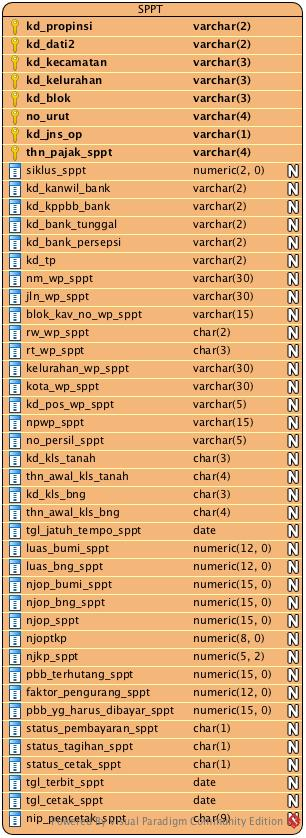
\includegraphics[width=0.5\textwidth]{./resources/struktur-tabel-sppt}
	\label{fig:struktur-tabel-sppt}
	\caption{Struktur Tabel \texttt{SPPT}}
\end{figure}

Pengambilan informasi pada tabel \texttt{SPPT} ini hanya beberapa \textit{field} atau kolom saja, yaitu :

\begin{itemize}
	\item Nomor Objek Pajak, yang terdiri dari \textit{field} atau kolom \texttt{kd\_propinsi}, \texttt{kd\_dati2}, \texttt{kd\_kecamatan}, \texttt{kd\_kelurahan}, \texttt{kd\_blok}, \texttt{no\_urut}, dan \texttt{kd\_jns\_op}.
	\item Tahun pajak pada \textit{field} atau kolom \texttt{thn\_pajak\_sppt}
	\item Nama wajib pajak pada \textit{field} atau kolom \texttt{nm\_wp\_sppt}
	\item Besarnya pajak terhutang pada \textit{field} atau kolom \texttt{pbb\_yg\_harus\_dibayar\_sppt}
	\item Status pembayaran pada \textit{field} atau kolom \texttt{status\_pembayaran\_sppt}
\end{itemize}

\subsection{Tabel DAT\_OBJEK\_PAJAK}

Tabel \texttt{DAT\_OBJEK\_PAJAK}, digunakan untuk menampilkan informasi mengenai objek pajak seperti alamat, luas bumi dan bangunan, serta Nilai Jual Objek Bumi dan Bangunan. Struktur tabel dari \texttt{DAT\_OBJEK\_PAJAK} adalah seperti pada gambar \ref{fig:struktur-dat-op} berikut ini :

\begin{figure}[H]
	\centering
	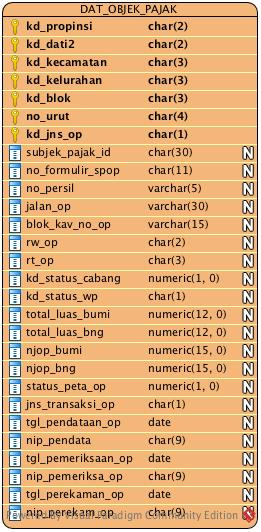
\includegraphics[width=0.5\textwidth]{./resources/struktur-tabel-dat-op}
	\caption{Struktur Tabel \texttt{DAT\_OBJEK\_PAJAK}}
	\label{fig:struktur-dat-op}
\end{figure}

Pengambilan informasi pada tabel \texttt{DAT\_OBJEK\_PAJAK} ini pada beberapa \textit{field} atau kolom seperti berikut :

\begin{itemize}
	\item Alamat, akan menggunakan gabungan dari \textit{field} atau kolom \texttt{jalan\_op}, \texttt{blok\_kav\_no\_op}, \texttt{rw\_op}, dan \texttt{rt\_op}.
	\item Luas bumi akan menggunakan \textit{field} atau tabel \texttt{total\_luas\_bumi}.
	\item Luas bangunan akan menggunakan \textit{field} atau tabel \texttt{total\_luas\_bng}.
	\item Nilai Jual Objek Pajak (NJOP) bumi akan menggunakan \textit{field} atau tabel \texttt{njop\_bumi}.
	\item Nilai Jual Objek Pajak (NJOP) bangunan akan menggunakan \textit{field} atau tabel \texttt{njop\_bng}.
\end{itemize}

\subsection{Tabel DAT\_SUBJEK\_PAJAK}

Tabel \texttt{DAT\_SUBJEK\_PAJAK} ini digunakan untuk menampilkan informasi mengenai subjek pajaknya seperti nama dan alamatnya. Struktur tabel dari \texttt{DAT\_SUBJEK\_PAJAK} ini adalah seperti pada gambar \ref{fig:struktur-dat-sp} berikut ini :

\begin{figure}[H]
	\centering
	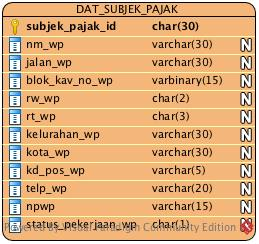
\includegraphics[width=0.5\textwidth]{./resources/struktur-tabel-dat-sp}
	\caption{Struktur Tabel \texttt{DAT\_SUBJEK\_PAJAK}}
	\label{fig:struktur-dat-sp}
\end{figure}

Informasi pada tabel \texttt{DAT\_SUBJEK\_PAJAK} yang digunakan ada pada beberapa \textit{field} atau kolom berikut :

\begin{itemize}
	\item Nama subjek pajak pada \textit{field} atau kolom \texttt{nm\_wp}
	\item Alamat subjek pajak pada \textit{field} atau kolom \texttt{jalan\_wp}, \texttt{blok\_kav\_no\_wp}, \texttt{rw\_wp}, \texttt{rt\_wp}, \texttt{kelurahan\_wp}, dan \texttt{kota\_wp}.
\end{itemize}

\subsection{Tabel REF\_KECAMATAN}

Untuk tabel \texttt{REF\_KECAMATAN} digunakan hanya untuk menampilkan informasi nama Kecamatan dimana objek berada. Struktur tabel untuk \texttt{REF\_KECAMATAN} ini seperti terlihat pada gambar \ref{fig:struktur-ref-kec} berikut ini :

\begin{figure}[H]
	\centering
	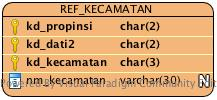
\includegraphics[width=0.5\textwidth]{./resources/struktur-tabel-ref-kec}
	\caption{Struktur Tabel \texttt{REF\_KECAMATAN}}
	\label{fig:struktur-ref-kec}	
\end{figure}

Informasi yang digunakan pada tabel \texttt{REF\_KECAMATAN} ini ada pada beberapa \textit{field} atau kolom berikut ini :

\begin{itemize}
	\item Nomor Identifikasi Kecamatan, pada \textit{field} atau kolom \texttt{kd\_propinsi}, \texttt{kd\_dati2}, dan \texttt{kd\_kecamatan}.
	\item Nama Kecamatan, pada \textit{field} atau kolom \texttt{nm\_kecamatan}
\end{itemize}

\subsection{Tabel REF\_KELURAHAN}

Tabel \texttt{REF\_KELURAHAN} pun digunakan hanya untuk menampilkan nama Kelurahan / Desa dimana objek pajak berada. Struktur tabel \texttt{REF\_KELURAHAN} ini seperti terlihat pada gambar \ref{fig:struktur-ref-kel} berikut ini :

\begin{figure}[H]
	\centering
	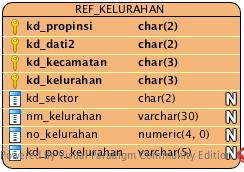
\includegraphics[width=0.5\textwidth]{./resources/struktur-tabel-ref-kel}
	\caption{Struktur Tabel \texttt{REF\_KELURAHAN}}
	\label{fig:struktur-ref-kel}
\end{figure}

Informasi pada tabel \texttt{REF\_KELURAHAN} yang digunakan ada pada beberapa \textit{field} atau kolom berikut ini :

\begin{itemize}
	\item Nomor Identifikasi Kelurahan / Desa pada \textit{field} atau kolom \texttt{kd\_propinsi}, \texttt{kd\_dati2}, \texttt{kd\_kecamatan}, dan \texttt{kd\_kelurahan}.
	\item Nama Desa / Kelurahan pada \textit{field} atau kolom \texttt{nm\_kelurahan}
\end{itemize}

\section{Hubungan Antar Entitas}

Dari tabel-tabel yang terbentuk pada bagian sebelumnya, dalam sistem ini akan membentuk sebuah jaringan relasi antar tabel dengan bentuk seperti pada gambar \ref{fig:db-diagram} berikut ini :

\begin{figure}[H]
	\centering
	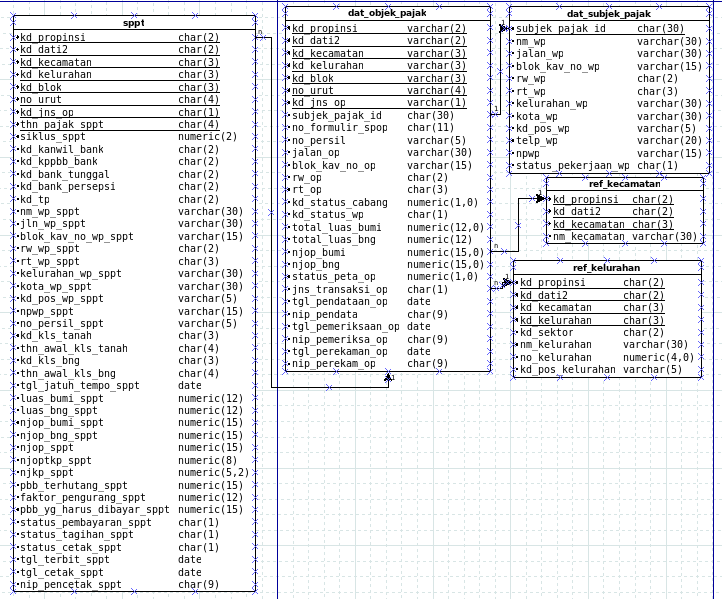
\includegraphics[width=0.5\textwidth]{./resources/db-diagram}
	\caption{Diagram Relasi \textit{Entity}}
	\label{fig:db-diagram}
\end{figure}

Titik utama akses aplikasi ini ada pada tabel \texttt{SPPT}, dimana nantinya tiap data pada tabel ini akan memiliki relasi n:1 dengan tabel \texttt{DAT\_OBJEK\_PAJAK}, ini karena tiap objek pajak yang tercatat akan memiliki banyak data SPPT untuk tiap tahun pajak.

Setiap data pada tabel \texttt{DAT\_OBJEK\_PAJAK} akan memiliki relasi 1:1 dengan data pada tabel \texttt{DAT\_SUBJEK\_PAJAK}. 

Sedangkan hubungan atau relasi antara tabel \texttt{DAT\_OBJEK\_PAJAK} dengan \texttt{REF\_KECAMATAN} dan \texttt{DAT\_OBJEK\_PAJAK} dengan \texttt{REF\_KELURAHAN} adalah n:1, dimana tiap 1 (satu) data pada tabel \texttt{REF\_KECAMATAN} atau \texttt{REF\_KELURAHAN} akan memiliki banyak objek pada tabel \texttt{DAT\_OBJEK\_PAJAK}.
\chapter{KEAMANAN \textit{DATABASE}}

Rancangan keamanan yang dilakukan pada sistem basis data, harus dapat menjamin ketersediaan, kehandalan, dan integritas layanan dari sistem basis data itu sendiri. Rancangan tersebut melihat dari beberapa poin penting yang diberikan adalah seperti berikut :

\section{Ketersediaan}

Ketersediaan koneksi atau sambungan ke sistem basis data menggunakan protokol TCP/IP dengan nomor \textit{port} 1521, untuk terhubung dengan sistem basis data, aplikasi perlu melakukan \textit{login} dengan menggunakan nama pengguna dan kata kunci (\textit{password}).

Nama pengguna dan kata kunci akan terbagi menjadi 2 (dua) bagian, yang pertama adalah nama pengguna dan kata kunci yang akan digunakan oleh aplikasi untuk \textit{login} ke dalam sistem basis data. Sedangkan nama pengguna dan kata kunci yang kedua digunakan oleh tiap pengguna yang diberikan akses untuk melakukan \textit{login} ke dalam aplikasi, pembatasan operasi akan dilakukan pada tingkat atau lapisan ini.

\section{Kehandalan}

Dari sisi kehandalan, sistem basis data memiliki fitur \textit{flash recovery area}, yang fungsinya adalah apabila ada kesalahan operasi terhadap data pada sistem basis data, data masih dapat dikembalikan berdasarkan waktu terjadinya perubahan / operasi data.

Kondisi lain yang dapat dilakukan pada fitur \textit{flash recovery area} adalah mampu melakukan \textit{recovery} atau pemulihan data per tanggal dan jam yang diinginkan dengan kondisi sistem basis data dalam keadaan melayani.

\section{Integritas Layanan}

Kondisi integrasi layanan untuk sistem basis data ini dilakukan melalui protokol TCP/IP dengan \textit{port} 1521. Parameter lain yang digunakan untuk terhubung dengan sistem basis data ini adalah \textit{tnsnames} dengan nama SID \texttt{sismiop}.
\chapter{KAPASITAS SISTEM BASIS DATA}

Kapasitas sistem basis data ini sebetulnya adalah sebesar kapasitas media simpanan atau \textit{disk} untuk data yang ada yaitu sebesar 1,22 TB (\textit{Tera Byte}). Sedangkan kapasitas untuk media \textit{backup} data adalah sebesar 279 GB (\textit{Giga Byte}).

Untuk kapasitas \textit{flash recovery area} disediakan ruang sebesar 65 GB (\textit{Giga Byte}) yang secara berkala harus dibersihkan agar kondisi operasional sistem basis data dapat berjalan dan diakses sebagaimana mestinya.

\backmatter%%%%%%%%%%%%%%%%%%%%%%%%%%%%%%%%%%%%%%%%%%%%%%%%%%%%%%%
\printindex

%%%%%%%%%%%%%%%%%%%%%%%%%%%%%%%%%%%%%%%%%%%%%%%%%%%%%%%%%%%%%%%%%%%%%%

\end{document}





